Una vez que demostramos tanto la correctitud como la complejidad temporal de nuestro algoritmo, pasamos a la fase de experimentación. En esta sección vamos a comprobar empíricamente que nuestro algoritmo tiene una complejidad temporal de $O(n^3)$, así como también mostrar como resolvemos algunos casos interesantes.

En este primer caso utilizamos instancias aleatorias, con distintos $n$ (es decir, variando en la cantidad total de cartas).

\begin{figure}[H]
  \begin{minipage}{0.5\linewidth}
    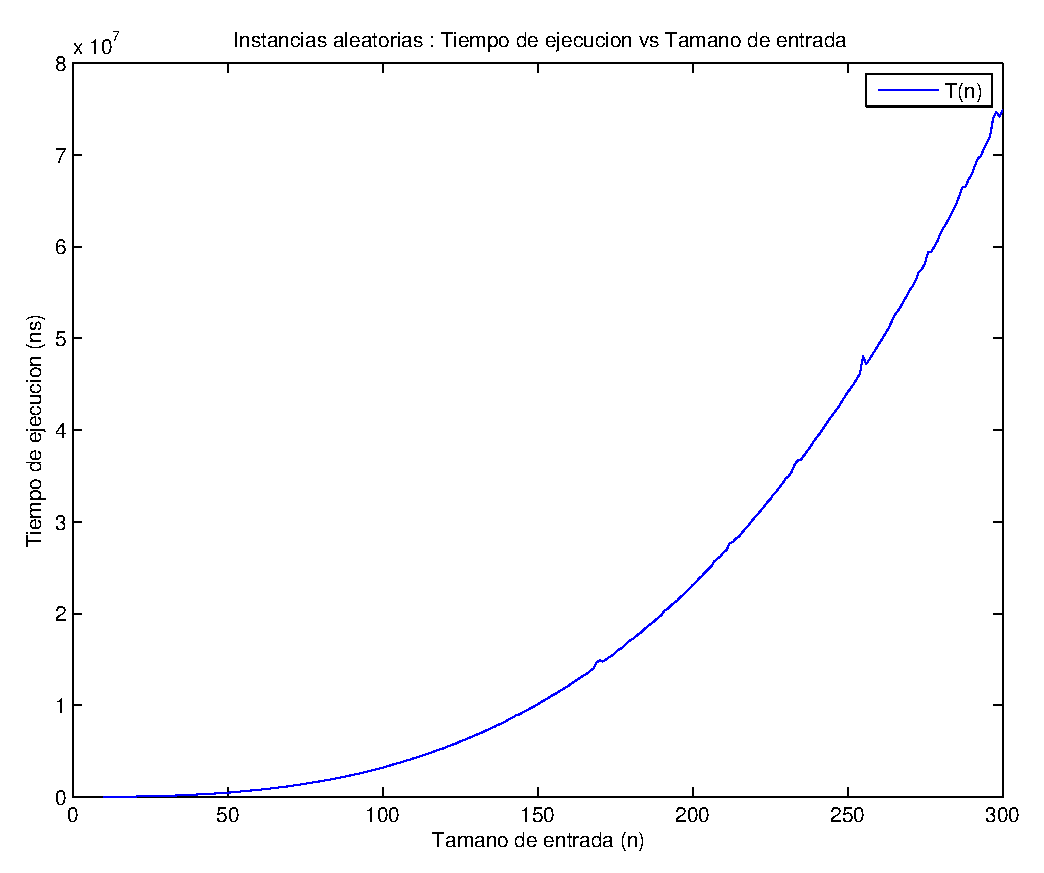
\includegraphics[width=\linewidth]{img/problema1/instancia_aleatoria.eps}
    \caption{Tiempo de ejecución instancia aleatoria}\label{fig:problema1-aleatoria}
  \end{minipage}
  \hfill
  \begin{minipage}{0.5\linewidth}
    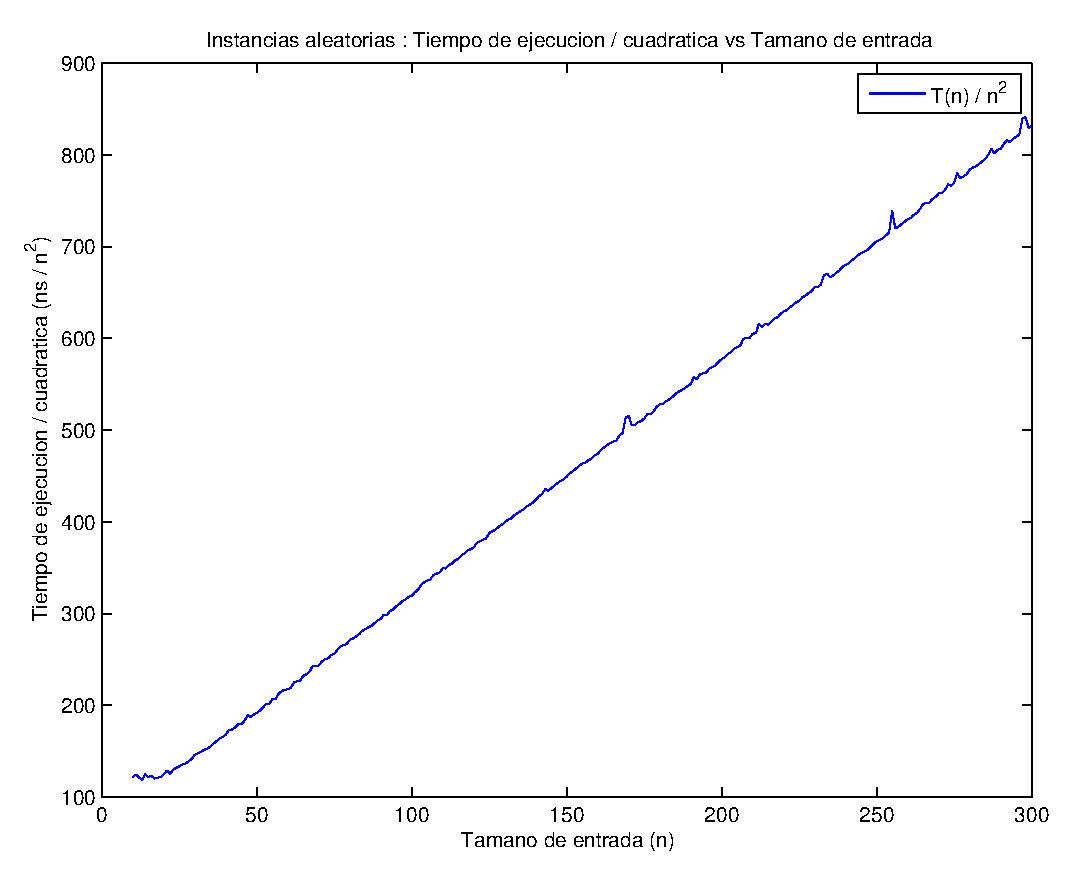
\includegraphics[width=\linewidth]{img/problema1/instancia_aleatoria_div_n2.eps}
    \caption{Idem, dividido por $n^2$}\label{fig:problema1-aleatoria-n2}
  \end{minipage}
\end{figure}

En la figura \ref{fig:problema1-aleatoria} no podemos notar la complejidad temporal de la función. Por esto, dividimos por $n^2$ y plasmamos ese resultado en la figura \ref{fig:problema1-aleatoria-n2}. En esta última figura, vemos claramente que $T(n) / n ^ 2$ es una recta. De esta manera, pudimos comprobar que $T(n)$ tiene una complejidad temporal de $O(n^3)$. En la figura \ref{fig:problema1-aleatoria-n2} podemos observar unos picos pequeños. Luego de realizar la experimentación, deducimos que dichos picos existen debido al desalojo por parte del \emph{scheduler}.
